\documentclass{article}

\usepackage{graphicx}

\topmargin=-0.5cm
\leftmargin=-2cm
\rightmargin=0cm
\oddsidemargin=0cm
\evensidemargin=2cm
\textwidth=16.5cm
\textheight=20cm

\pagestyle{plain}

\begin{document}

\large

\vbox{}
\vspace{-2cm}
\begin{figure}[!ht]
%\hspace{-4mm}

\includegraphics[width=5cm]{img/logo.png}
\vspace{4mm}
\end{figure}
\noindent
\begin{center}
{\Huge Capacitor Module}\\[2mm]
Based on Hermes2D ({\tt http://hpfem.org/hermes})\\[6mm]
\end{center}
\section{Module Description}

The capacitor model calculates the distribution of the electric 
potential $\varphi$ induced by stationary electric charges on the two plates of the capacitor.
One first has to specify dimensions of the capacitor (the size of the plates $h$ and distance between the plates $d$).
Then the relative permittivity $\epsilon_r$ of the dielectric and voltages on the two plates need to be specified.

The image below shows a real-life plate capacitor with white-colored dielectric between the two plates.
 

\begin{figure}[!ht]
\begin{center}
%\hspace{-4mm}
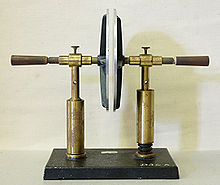
\includegraphics[width=10cm]{img/capacitor.png}
\caption{A plate capacitor.}
\vspace{4mm}
\end{center}
\end{figure}
\noindent


\section{Underlying Equations}

The equation for the electric potential $\varphi$ is 

$$
-\mbox{div}(\epsilon \nabla \varphi) = \varrho
$$
where $\varrho$ is electric charge density. Once the electric potential 
$\varphi$ is calculated, the electric field vector $E$ can be obtained
as its negative gradient,

$$
E = -\nabla \varphi.
$$

\end{document}

